% 2009 年江西卷文科第 20 题：四棱锥 P-ABCD，球心 O 为 BD 中点，球面交 PD 于 M。
% 来源 PDF：普通高考/2009/2009江西文.pdf，SHA-256 468ed0d312446a29e8cdaebe70fab4f803741b0b542cd991781b2f13fed5168f。
% 原页：第 2 页（A3 三栏）第 1 栏，书页码 536。
% 重绘依据：原图 P 在顶点，B 在左下、C 在右下、D 在右、A 在左后被遮挡；
%   PA、AB、AD、BD、AM、BM 为虚线，PB、PC、PD、BC、CD 为实线，O 为 BD 上的实心点，M 在 PD 上。
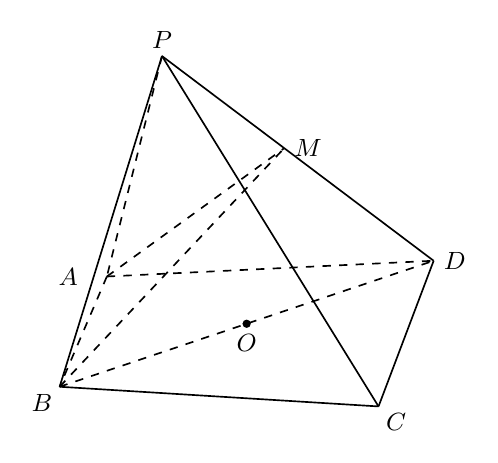
\begin{tikzpicture}[scale=1.0, semithick, every node/.style={inner sep=1.4pt, font=\small}]
  \coordinate (P) at (2.15,5.15);
  \coordinate (A) at (1.45,2.35);
  \coordinate (B) at (0.85,0.95);
  \coordinate (C) at (4.90,0.70);
  \coordinate (D) at (5.60,2.55);
  \coordinate (O) at (3.225,1.75);
  \coordinate (M) at (3.7025,3.98);

  % 可见棱
  \draw (P) -- (B);
  \draw (P) -- (C);
  \draw (P) -- (M) -- (D);
  \draw (B) -- (C);
  \draw (C) -- (D);

  % 被遮挡的棱与辅助线
  \draw[dashed] (P) -- (A);
  \draw[dashed] (A) -- (B);
  \draw[dashed] (A) -- (D);
  \draw[dashed] (B) -- (D);
  \draw[dashed] (A) -- (M);
  \draw[dashed] (B) -- (M);

  % 球心 O
  \fill (O) circle (1.5pt);

  \node[above=1pt] at (P) {$P$};
  \node[anchor=east] at (1.14,2.34) {$A$};
  \node[below left=1pt] at (B) {$B$};
  \node[below right=1pt] at (C) {$C$};
  \node[right=2pt] at (D) {$D$};
  \node[below=2pt] at (O) {$O$};
  \node[right=2pt] at (M) {$M$};
\end{tikzpicture}
